%\documentstyle[epsf,twocolumn]{jarticle}       %LaTeX2e仕様
\documentclass[twocolumn]{jarticle}     %pLaTeX2e仕様(platex.exeの場合)
% \documentclass[onecolumn]{ujarticle}   %pLaTeX2e仕様(uplatex.exeの場合)
%%%%%%%%%%%%%%%%%%%%%%%%%%%%%%%%%%%%%%%%%%%%%%%%%%%%%%%%%%%%%%
%%
%%  基本バージョン
%%
%%%%%%%%%%%%%%%%%%%%%%%%%%%%%%%%%%%%%%%%%%%%%%%%%%%%%%%%%%%%%%%%
\setlength{\topmargin}{-45pt}
%\setlength{\oddsidemargin}{0cm}
\setlength{\oddsidemargin}{-7.5mm}
%\setlength{\evensidemargin}{0cm}
\setlength{\textheight}{24.1cm}
%setlength{\textheight}{25cm}
\setlength{\textwidth}{17.4cm}
%\setlength{\textwidth}{172mm}
\setlength{\columnsep}{11mm}

%\kanjiskip=.07zw plus.5pt minus.5pt


% 【節が変わるごとに (1.1)(1.2) … (2.1)(2.2) と数式番号をつけるとき】
%\makeatletter
%\renewcommand{\theequation}{%
%\thesection.\arabic{equation}} %\@addtoreset{equation}{section}
%\makeatother

%\renewcommand{\arraystretch}{0.95} 行間の設定
%%%%%%%%%%%%%%%%%%%%%%%%%%%%%%%%%%%%%%%%%%%%%%%%%%%%%%%%
%\usepackage{graphicx}   %pLaTeX2e仕様(\documentstyle ->\documentclass)
\usepackage[dvipdfmx]{graphicx}
\usepackage{subcaption}
\usepackage{multirow}
\usepackage{amsmath}
\usepackage{url}
\usepackage{ulem}
\usepackage{algorithm}
\usepackage{algorithmic}
\usepackage{listings} %,jlisting} %日本語のコメントアウトをする場合jlistingが必要
%ここからソースコードの表示に関する設定
\lstset{
  basicstyle={\ttfamily},
  identifierstyle={\small},
  commentstyle={\smallitshape},
  keywordstyle={\small\bfseries},
  ndkeywordstyle={\small},
  stringstyle={\small\ttfamily},
  frame={tb},
  breaklines=true,
  columns=[l]{fullflexible},
  numbers=left,
  xrightmargin=0zw,
  xleftmargin=3zw,
  numberstyle={\scriptsize},
  stepnumber=1,
  numbersep=1zw,
  lineskip=-0.5ex
}
\newcommand{\argmax}{\mathop{\rm arg~max}\limits}
\newcommand{\argmin}{\mathop{\rm arg~min}\limits}

%%%%%%%%%%%%%%%%%%%%%%%%%%%%%%%%%%%%%%%%%%%%%%%%%%%%%%%%
\begin{document}

	%bibtex用の設定
	%\bibliographystyle{ujarticle}

	\twocolumn[
		\noindent
		\hspace{1em}
		2021 年 1 月 8 日
		ゼミ資料
		\hfill
		B4 杉山 竜弥
		\vspace{2mm}

		\hrule
		\begin{center}
			{\Large \bf 進捗報告}
		\end{center}
		\hrule
		\vspace{9mm}
	]

\section{今週やったこと}
\begin{itemize}
  \item TDGAの実装
\end{itemize}

\section{変更}

以前までブロック単位でSoftmaxしていた (\ref{equ:cut}) 式 を, 辺単位で正規化する (\ref{equ:cut_a}) 式 に変更してみた.
\begin{equation}
  \label{equ:cut}
  x_i = f^{\mathrm{c}}_{i-1, i}(x_{i-1}) + \beta_i \sum_{j \in S_i} \mathrm{Softmax} ( \alpha_{i})_j f^{\mathrm{s}}_{j, i} (x_j)
\end{equation}
\begin{equation}
  \label{equ:cut_a}
  x_i = f^{\mathrm{c}}_{i-1, i}(x_{i-1}) + \sum_{j \in S_i} \mathrm{Sigmoid} ( \alpha_{ij}) f^{\mathrm{s}}_{j, i} (x_j)
\end{equation}

これによって, $\beta$の補正がなくなり, 3本のショートカットができたり, 全体の本数が増えたりした.

\section{実験}

\begin{table}[tb]
  \begin{center}
    \caption{モデルの設定}
    \begin{tabular}{|c|c|} \hline
      base model & VGG19 \\ \hline
      Optim($w$) & SGD(lr=0.001, momentum=0.9) \\ \hline
      Optim($\alpha$) & Adam(lr=0.001, $\beta$=(0.5, 0.999)) \\ \hline
      Loss & Cross Entropy Loss \\ \hline
      dataset & cifar10 \\ \hline
      pretrain & true \\ \hline
      batch size & 64 \\ \hline
      train size & 12500 \\ \hline
      valid size & 5000 \\ \hline
    \end{tabular}
    \label{tab:setting}
  \end{center}
\end{table}

\begin{table}[tb]
  \begin{center}
    \caption{GAの設定}
    \begin{tabular}{|c|c|} \hline
      個体数 & 10 \\ \hline
      世代数 & 60 \\ \hline \hline
      選択 & TD選択 \\ \hline
      温度 & 10 $\rightarrow$ ?? \\ \hline \hline
      交叉 & 一様交叉 \\ \hline
      交叉率 & 0.5 (0.5) \\ \hline \hline
      変異 & ガウス分布 \\ \hline
      変異率 & 0.2 (0.2) \\ \hline
    \end{tabular}
    \label{tab:setting_ga}
  \end{center}
\end{table}

表 \ref{tab:setting}, \ref{tab:setting_ga} にモデルとGAの設定を示した.

(温度設定は, 10 $\rightarrow$ 2 $\rightarrow$ 1 にしたつもりが, 始点と終点がぐちゃぐちゃになっていた.)


\section{結果}

図 \ref{fig:graph} は最終世代の最良個体のグラフ, アーキテクチャの評価は 93.68 \%

図 \ref{fig:edge} はショートカット数の平均だが, 分散を保ちつつ減少方向へ学習できていることが分かる.

図 \ref{fig:acc} はテスト accuracy の平均を示す.
GAなしの実験時は 88 \% 程度だったのが, 82 \% 程度で伸びが悪い.
One Shotモデルで $w$ を共有しているため, それぞれの個体に引っ張られて学習が遅いと思われる.

\begin{figure}[tb]
  \begin{center}
    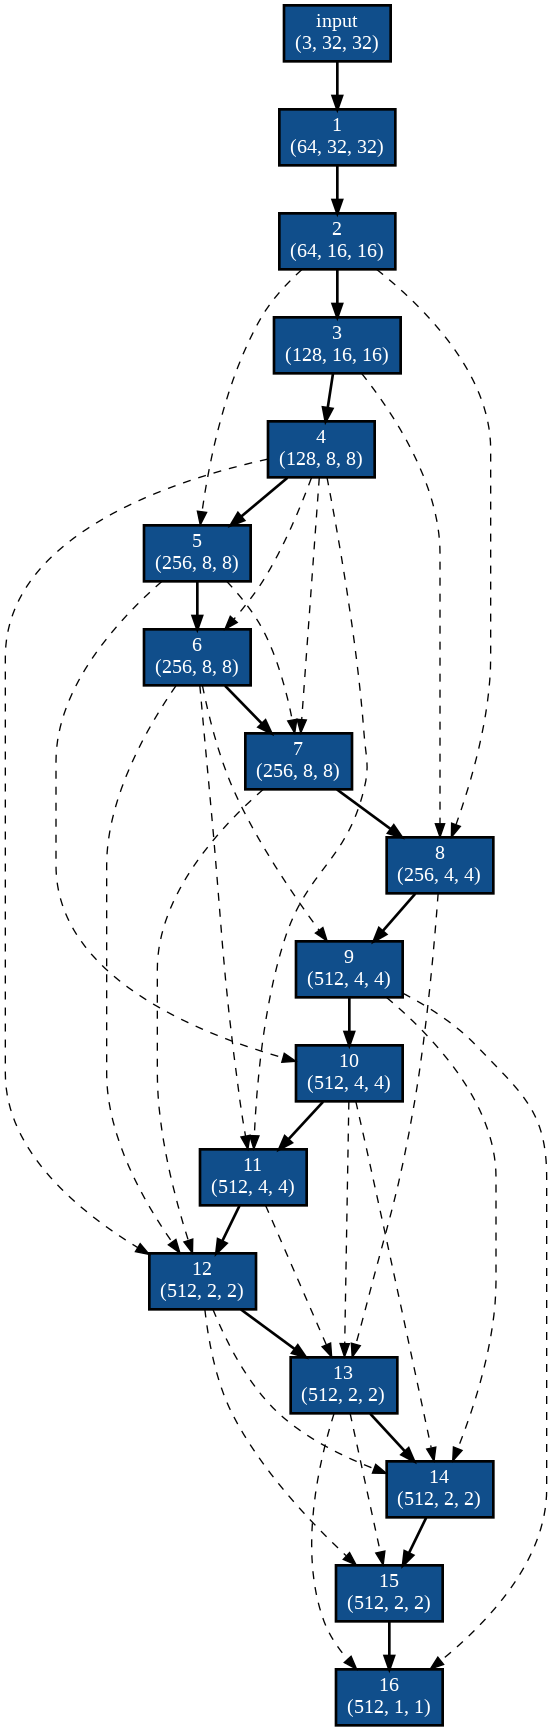
\includegraphics[clip,width=75mm]{graph_150.png}
    \caption{最終世代の最良個体のグラフ}
    \label{fig:graph}
  \end{center}
\end{figure}

\begin{figure}[tb]
  \begin{center}
    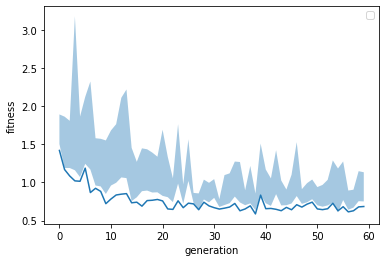
\includegraphics[clip,width=75mm]{fit.png}
    \caption{世代ごとの fitness}
    \label{fig:fit}
  \end{center}
\end{figure}

\begin{figure}[tb]
  \begin{center}
    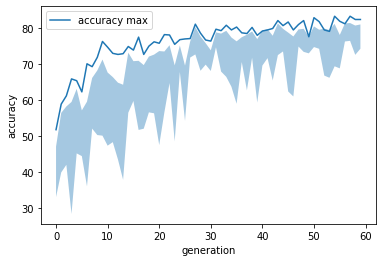
\includegraphics[clip,width=75mm]{acc.png}
    \caption{世代ごとの test accuracy}
    \label{fig:acc}
  \end{center}
\end{figure}

\begin{figure}[tb]
  \begin{center}
    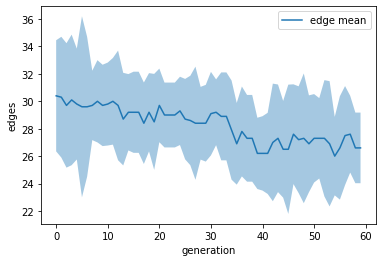
\includegraphics[clip,width=75mm]{edge.png}
    \caption{世代ごとのショートカット数}
    \label{fig:edge}
  \end{center}
\end{figure}


% \section{TDGA}
% $F$を最小化する.
% \begin{equation}
%   F = \langle E \rangle - HT
% \end{equation}
% \begin{equation}
%   H = \sum^{M}_{k=1} H_k,
% \end{equation}
% \begin{equation}
%   H_k = - \sum_{j} P^k_j log P^k_j
% \end{equation}
% エントロピー $H$ をグラフ用に改造する必要がある.
%
% 単純に考えるなら分散をとる?
% \begin{equation}
%   H = \frac{1}{|\mathcal{E}|} \sum_{i, j} ( \alpha_{ij} - \bar{\alpha}_{ij} )^2
% \end{equation}
% $|\mathcal{E}|$はDARTSの辺の数
%
% \subsection{分からなかった点}
% \begin{equation}
%   \mathcal{P}(t+1, i, h) \Leftarrow \mathcal{P}(t+1) \cup \{h\}
% \end{equation}
% \begin{equation}
%   F_h = \langle E_{\mathcal{P}(t+1, i, h)} \rangle - H_{\mathcal{P}(t+1, i, h)}T
% \end{equation}
% \begin{equation}
%   \label{equ:mi}
%   h_{\min} \Leftarrow \argmin_h F_h
% \end{equation}
% \begin{equation}
%   \mathcal{P}(t+1) \Leftarrow \mathcal{P}(t+1) \cup \{h_{\min}\}
% \end{equation}
% (\ref{equ:mi}) 式は
% どうやって $h$ を選んでいるのか.
% $h$ は重複するのか

\section{今後の予定}
% なんとなくなんかの勉強をするとかではなく具体的に
\begin{itemize}
  \item 動作は確認できたので, 世代数を増やすなどのパラメータの見直しを検討.
  \item 卒論の準備.

\end{itemize}

% 参考文献リスト
\bibliographystyle{unsrt}
\bibliography{ref}
\end{document}
